\subsection{Previous Work}

\paragraph{Linux Kernel Scalability} Operating system kernel schedules the
execution of multithreaded programs and handles I/O requests for 
applicaitons. Silas\cite{rel:silas} suggested in his paper that potential
careless code in kernel code could significantly limit the parallelism of 
multithreaded programs. They have studied the scalability of some popular 
parallel applications on Linux Kernel and pointed out some issues that 
limit parallelism.
\begin{center}
\begin{tabular}[t] {l|l} 
Application & Bottleneck \\
\hline
Exim &App: Contention on spool directories \\
memcached &HW: Transmit queues on NIC \\
Apache &HW: Receive queues on NIC \\
PostgreSQL &App: Application-level spin lock \\
gmake &App: Serial stages and stragglers \\
pedsort &HW: Cache capacity \\
Metis &HW: DRAM throughpu 
\end{tabular}
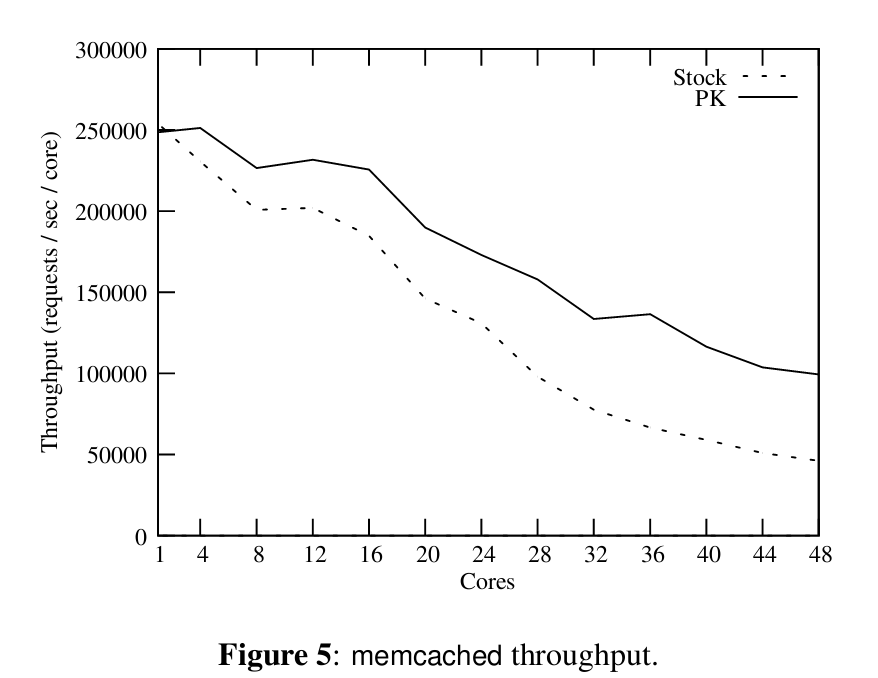
\includegraphics[width=0.8\linewidth]{figures/memcachced_scal.png}
\end{center}

%In subsections there is 1 blank line before the section 
%heading and one afterwards.  Heading text is 11 point 
%bold font.  Paragraphs are indented one pica.  There is 
%no blank line between paragraphs.
%Throughout I may cite references of the form 
%\cite{key:foo} or \cite{foo:baz}, and LaTeX will keep 
%track of numbering.  The numbers are based on the order 
%you place them in the bibliography, not the order they 
%appear in the text.  They should (I believe) be in 
%alphabetical order.  LaTex will put square brackets about 
%the number within the text of your paper.  For those of 
%you new to the bibliography package, you may have to run 
%the latex process twice to allow all references to be 
%resolved. You will get a warning about a missing .aux 
%file.  Just rerun latex and it will be ok.
%
